% !TEX root = ../Micro.tex
\chapter{Introduction}

\rmkb[Reading This Chapter]{
  This chapter is informal motivation, not formal theory. Three short vignettes---a traffic network, a guessing game, a model of herding---preview the recurring themes of strategic interaction, information, and equilibrium that the rest of the book develops rigorously. Formal definitions begin in Chapter~2.
}

\ex[Braess' Paradox]{
\begin{center}
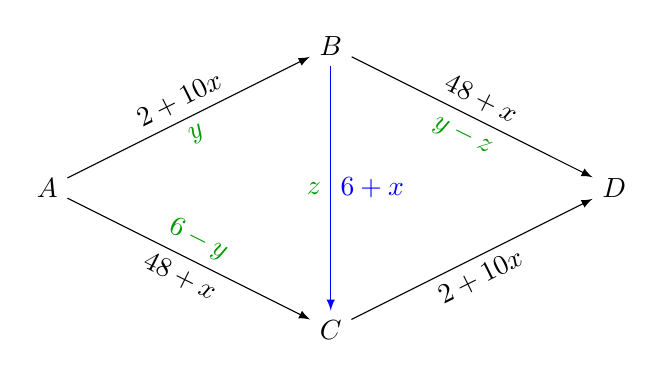
\begin{tikzpicture}[
    scale=0.9,               % 调整整体大小
    >={latex}
]

    % --- 1. 定义节点位置 (Nodes) ---
    \node (A) at (0, 0) {$A$};
    \node (B) at (4, 2) {$B$};
    \node (C) at (4, -2) {$C$};
    \node (D) at (8, 0) {$D$};

    % --- 2. 绘制黑色路径 (Black Edges) ---

    % A -> B (Top Left)
    % 黑色文字在上方，绿色流量 y 在下方
    \draw[->] (A) --
        node[above, sloped] {$2+10x$}
        node[below, sloped, text=green!60!black] {$y$}
        (B);

    % A -> C (Bottom Left)
    % 黑色文字在下方，绿色流量 6-y 在上方 (原图中写的是 6-y 或 b-y，此处按流量守恒推断为 6-y)
    \draw[->] (A) --
        node[below, sloped] {$48+x$}
        node[above, sloped, text=green!60!black] {$6-y$}
        (C);

    % B -> D (Top Right)
    % 黑色文字在上方，绿色流量 y-z 在下方
    \draw[->] (B) --
        node[above, sloped] {$48+x$}
        node[below, sloped, text=green!60!black] {$y-z$}
        (D);

    % C -> D (Bottom Right)
    % 黑色文字在下方 (原图中这部分似乎没有标绿色流量，如果需要可以加上)
    \draw[->] (C) --
        node[below, sloped] {$2+10x$}
        (D);

    % --- 3. 绘制蓝色捷径 (Blue Shortcut) ---

    % B -> C (Middle)
    % 蓝色箭头，右侧标成本，左侧标绿色流量 z
    \draw[->, blue] (B) --
        node[right] {$6+x$}
        node[left, text=green!60!black] {$z$}
        (C);

\end{tikzpicture}
\end{center}

The core idea to solve for equilibrium is that, in equilibrium, costs (the time spent on each possible route from $A$ to $D$) must be equal on all paths. Before the shortcut is connected, the equilibrium travel time for any driver is $83$ minutes. After the shortcut is built, the new equilibrium travel time becomes $92$, which is actually greater than the original.

In the example, although the network capacity increased by adding the shortcut, the individual cost for every agent increased. This is due to the negative externality: when an agent switches to the shortcut, they reduce their own time marginally but impose a heavy congestion cost on the shared links $AB$ and $CD$. This cost is not internalized by the selfish agents.
}

\rmkb{
  \begin{itemize}
    \item In a multi-agent situation, having more choices can make you (and even everyone) worse off.
    \item In a single-person decision problem, however, having more choices always makes you at least as well off.
  \end{itemize}
}

\ex[Coin Toss with Sequential Moves]{
Agent A announces her guess first; B announces hers after observing A's. If both agents make the same guess, both get $1$. Otherwise, nature determines the winner by coin toss: whichever guess matches the coin toss wins $4$, the other gets $0$.
\[
\begin{array}{cccc}
\text{Coin} & A & B & \text{Payoff} \\
\hline
H & H & H & (1,1) \\
T & H & H & (1,1) \\
H & T & T & (1,1) \\
T & T & T & (1,1) \\
H & H & T & (4,0) \\
H & T & H & (0,4) \\
T & H & T & (0,4) \\
T & T & H & (4,0) \\
\end{array}
\]

If the coin toss is unavailable to both of them, B will make a guess opposite to $A$'s as long as $B$ is not too risk-averse. The expected payoff is $(2,2)$.

If instead the coin toss is observed by $A$ and this is common knowledge, $A$'s best strategy is to guess consistently with the actual coin toss, and $B$'s best response is to report the same as $A$. Both then receive a certain payoff of $(1,1)$.
}

\rmkb{
  Information can have negative value! In the example, making the coin toss \emph{commonly known} to be observed by $A$ actually hurts $A$. By contrast, if the revelation is $A$'s \emph{private} knowledge, the information must have nonnegative value.
}

\ex[Herding via Information Cascades]{
Suppose there are two restaurants in a town, $A$ and $B$, with common prior
\[
\Pr{A>B} = p>\frac{1}{2},
\]
where $A>B$ denotes the event that restaurant $A$ is better than $B$. Everyone is therefore mildly inclined toward $A$ absent further information. Two private signals $\alpha$ and $\beta$ are available, with
\[
\begin{aligned}
  \Pr{\alpha|A>B} = q,\\
  \Pr{\beta|B>A} = q,
\end{aligned}
\]
where $q>\frac{1}{2}$ and $q>p$.\footnote{
  $q>p$ ensures that an agent observing a signal contrary to the prior forms a posterior favoring the signal over the prior.
}

The $t$-th agent observes all $(t-1)$ prior agents' choices but not their private signals.

Suppose the realized signal sequence is $(\alpha,\beta,\beta,\ldots,\beta)$.

\smallskip
\emph{Agent 1.} Receives $\alpha$, which reinforces the prior. Since $\Pr{A>B|\alpha} > \frac{1}{2}$, she chooses $A$.

\emph{Agent 2.} Infers from Agent 1's choice that Agent 1 must have received $\alpha$. Agent 2's own signal is $\beta$. The two signals cancel out,\footnote{
  Verifiable by Bayes' rule:
  \[
  \begin{aligned}
    \Pr{A>B|\alpha,\beta} &= \frac{\Pr{\alpha,\beta|A>B}\Pr{A>B}}{\Pr{\alpha,\beta|A>B}\Pr{A>B} + \Pr{\alpha,\beta|B>A}\Pr{B>A}}\\
    &= \frac{q(1-q) \cdot p}{q(1-q) \cdot p + (1-q)q \cdot (1-p)}\\
    &= p > \frac{1}{2}.
  \end{aligned}
  \]
  Hence Agent 2's posterior coincides with the prior, as if she had received no informative evidence.
} so the prior dictates: Agent 2 also chooses $A$.

\emph{Agent 3.} Infers Agent 1's $\alpha$ from her choice. For Agent 2: if Agent 2 had $\alpha$, Agent 2 would have chosen $A$; if Agent 2 had $\beta$, the two signals would cancel and Agent 2 would still choose $A$ by the prior. So Agent 2's choice is \emph{uninformative} about her private signal. Agent 3 therefore only learns $s_1 = \alpha$ from history; combined with her own $s_3 = \beta$, the two cancel and Agent 3 chooses $A$.

\smallskip
The same logic propagates: every subsequent agent ignores her private signal and chooses $A$. This is the \emph{herding} phenomenon---an information cascade in which collective behavior locks onto the prior despite a sequence of contrary private signals.
}

\rmkb{
  \begin{itemize}
    \item The assumption $q>p$ matters because it ensures
  \[
  \begin{aligned}
    \Pr{B>A|\beta} & = \frac{\Pr{\beta|B>A}\Pr{B>A}}{\Pr{\beta|B>A}\Pr{B>A} + \Pr{\beta|A>B}\Pr{A>B}} \\
    & = \frac{q(1-p)}{q(1-p)+(1-q)p}>\frac{1}{2}.
  \end{aligned}
  \]
  (Similarly, $\Pr{A>B|\alpha}>\frac12$.) So a single private signal is strong enough to overturn the prior. Without this assumption agents would be ``blinded'' by the prior and ignore their signals from the start---no cascade would form because there was never any private content to suppress.

    \item Even with strong signals, the cascade is not perfect. Starting from Agent 2, the information aggregation breaks down: each agent's choice no longer reveals her private signal.

    \item Agent 2 cares only about her own payoff. If she also cared about social welfare, she would choose according to her private signal (i.e., $B$ if she received $\beta$) to reveal her information to subsequent agents. There is no individual incentive to do so---an information externality that leads to inefficiency.
  \end{itemize}
}
